\chapter{An Example Yocto Project Set up} \label{yocto-setup}

Consider a simple development scenario targetting the embedded hardware device MCIMX6Q-SDB, the primary hardware utilized for this report. The aim is to build and run an Embedded Linux distribution for the MCIMX6Q-SDB using a personal computer running Linux. Note that several of the code listings used in this discussion may break their interface, hence the emphasis is primarily on the essential concepts involved.

The primary version control system used within the Yocto Project is git. The Yocto Project has several other software packages that are required for its build system, all of which are laid out in its documentation (see \href{https://docs.yoctoproject.org/}{docs.yoctoproject.org}). Furthermore, there are minimum versions for the required packages for a given version of its release (see \href{https://wiki.yoctoproject.org/wiki/Releases}{wiki.yoctoproject.org/wiki/Releases}).

The following listing presents the typical required packages however, based on the Linux distribution of the development host the command will vary.

\begin{minted}[bgcolor=lightgray]{bash}
PACKAGE_MANAGER install bc make automake gcc gcc-c++ chrpath cpio diffstat gawk git python texinfo wget zstd lz4
\end{minted}

The above list is an incomplete example and relies on non-standard package names. Consulting the Yocto Project documentation provides a more accurate instruction as to the package names that are necessary to start with the Yocto Project on a given Linux distribution. An example install of the packages necessary on the Fedora 37 operating system as recommended by the Yocto Project documentation is given in the following code listing. Note that the listing assumes certain administrative capabilities to successfully complete its execution.

\begin{minted}{bash}
sudo dnf install gawk make wget tar bzip2 gzip python3 unzip perl patch diffutils diffstat git cpp gcc gcc-c++ glibc-devel texinfo chrpath ccache perl-Data-Dumper perl-Text-ParseWords perl-Thread-Queue perl-bignum socat python3-pexpect findutils which file cpio python python3-pip xz python3-GitPython python3-jinja2 SDL-devel rpcgen mesa-libGL-devel perl-FindBin perl-File-Compare perl-File-Copy perl-locale zstd lz4 hostname glibc-langpack-en
\end{minted}

For this section, consider the \textit{kirkstone} Long Term Support (LTS) release of the Yocto Project. To begin clone the Poky repository from \href{https://git.yoctoproject.com}{git.yoctoproject.com}

\begin{minted}{bash}
git clone https://git.yoctoproject.org/git/poky
\end{minted}

The Poky repository contains the OpenEmbedded-Core as well as the BitBake tool that is required for the build. NXP (previously \textit{freescale}) is the system maker and system vendor for the MCIMX6Q-SDB, and they provide a BSP layer in Yocto via the meta-freescale repository.

\begin{minted}{bash}
git clone https://git.yoctoproject.org/git/meta-freescale
\end{minted}

Checkout the kirkstone version of the different components by checking out the corresponding branches of the git repos. Using a different version of the Yocto Project would primarily mean checking out to a different branch or tag at this point.

\begin{minted}{bash}
git checkout kirkstone-4.0.11 # for poky
\end{minted}

\begin{minted}{bash}
git checkout kirkstone # for meta-freescale
\end{minted}

Once the correct branches have been checked out, the next step is to bring the BitBake tool into the shell environment. The Poky repository contains scripts that facilitate this step. Create a directory (assumed that \texttt{\$BUILDDIR} holds the pathname) to manage the build configuration and output files, and run the setup script inside the Poky repo.

\begin{minted}{bash}
source poky/oe-init-build-env $BUILDDIR
\end{minted}

The script will set up BitBake along with some additional tools and scripts in the current shell environment and also creates a few directories in \texttt{\$BUILDDIR} along with some configuration files. Note that after sourcing the \texttt{oe-init-build-env} script, the shell switches to the \texttt{\$BUILDDIR} directory. The first configuration file to edit will be the \texttt{\$BUILDDIR/conf/bblayers.conf}. The \texttt{bblayers.conf} file contains a list of layers to be used in the Yocto Project set up. The \texttt{bitbake-layers} utility program can be used to list and modify the entries in the \texttt{bblayers.conf} file.

\begin{minted}{bash}
bitbake-layers show-layers # list layers in the Yocto Project set up
\end{minted}

The above code listings shows \texttt{bitbake-layers} being used to list the layers of Yocto Project set up. The command should then list the \texttt{meta}, \texttt{meta-poky}, and \texttt{meta-yocto-bsp} layers. The names of the layers may change with the particular version of the Yocto Project being used. The path corresponding to those layers and a priority value attached to the layers will also be shown by the \texttt{show-layers} command of \texttt{bitbake-layers}. The priority is a means for BitBake to choose between layers for searching a recipe for particular software package, since multiple layers may have instructions for the same package. The \texttt{meta-freescale} layer that was cloned in the previous command to some path \texttt{\$META\_FREESCALE\_PATH} can then be added to the Yocto Project configuration using the same utility.

\begin{minted}{bash}
bitbake-layers add-layer $META_FREESCALE_PATH
\end{minted}

The next step is to configure the build system for the MCIMX6Q-SDB. The Note that this step may also be avoided by setting the \texttt{\$MACHINE} environment variable.

\begin{minted}{bash}
# edit inside $BUILDDIR/conf/local.conf
MACHINE = "imx6qdlsabresd"
\end{minted}

After \texttt{\$MACHINE} is configured correctly, BitBake can create a minimal image that can boot the MCIMX6Q-SDB by building the packages for \texttt{core-image-minimal} recipe. BitBake can parse a recipe file to determine a series of tasks to generate a software package or some binary artefacts. To satisfy the \texttt{core-image-minimal} recipe, BitBake has to perform a series of operations. BitBake has to parse a list of recipe files that are associated with the \texttt{core-image-minimal} recipe, examine the dependencies defined in the recipes and recursively determine all the software components that are required.

\begin{minted}{bash}
bitbake core-image-minimal # generate images for MCIMX6Q-SDB
\end{minted}

At this point the Yocto Project has been configured to find the correct metadata for building software packages and the Linux kernel for the MCIMX6Q-SDB. BitBake will proceed by first going through the \texttt{core-image-minimal} recipe to determine the order and list of tasks to be executed. After listing some information on the particular build configuration, it will then proceed to execute the tasks. The generated output images can be found in \texttt{\$BUILDDIR/tmp/deploy/images}. The path ends at the same name as the \texttt{\$MACHINE} variable name and contains several binary images. One way to use the resulting binary images to boot the MCIMX6Q-SDB is to use an SD card and the \textit{rootfs} image. The rootfs image should be named with the name of the machine, a time stamp, and the string \texttt{"rootfs"}.

\begin{figure}[h]
	\centering
	\begin{tikzpicture}
		\node (image) at (0, 0)
			{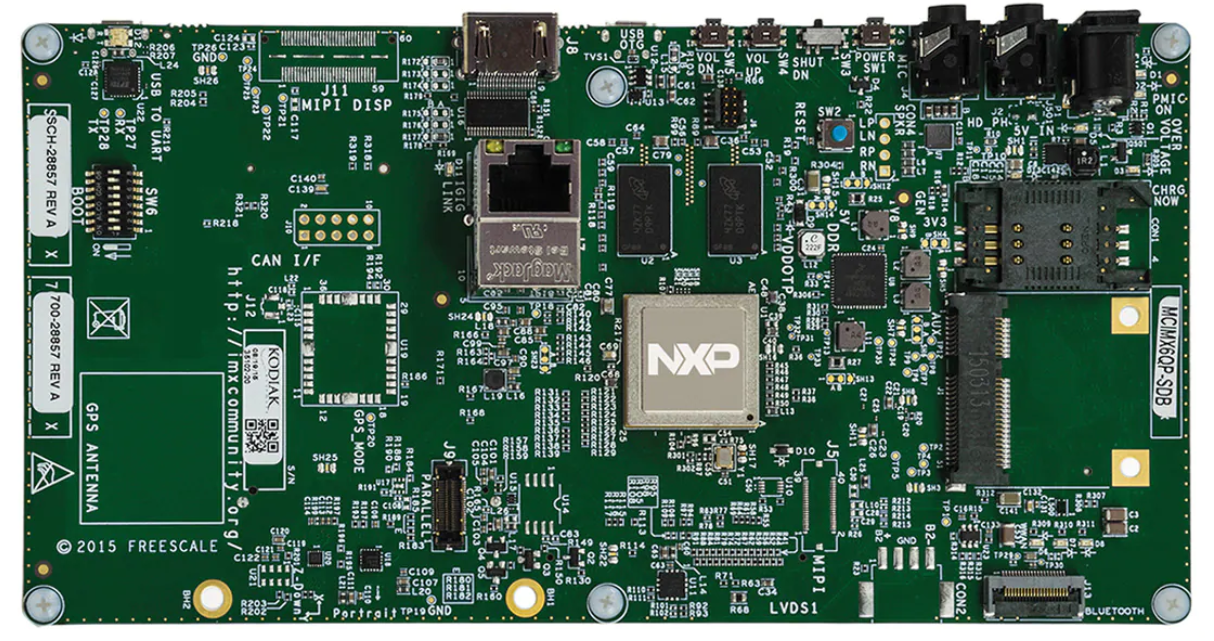
\includegraphics[scale=0.34]{MCIMX6Q-SDB-BD.png}};
		\draw[rounded corners=1ex, line width=2.1pt, yellow] (-6.5, 0.7) rectangle (-5.2, 1.9);
	\end{tikzpicture}
	\caption{MCIMX6Q-SDB-BD}
	\label{fig:mcimx6q-sdb}
\end{figure}

Booting the board using this image is one way to verify the build completed by BitBake. Obtain and flash an SD card with the \textit{rootfs} image using a suitable program such as \texttt{dd}. Furthermore, the MCIMX6Q-SDB should be configured to boot from an SD card slot. The board can be configured to boot from the SD-3 slot by toggling the dip switches (shown in yellow highlights in Figure \ref{fig:mcimx6q-sdb}) to the configuration : \texttt{D1-OFF D2-ON D3,4,5,6-OFF D7-ON D8-OFF}.

Assuming the previous steps were completed in a correct manner, the board should boot using the Embedded Linux that was created by BitBake using the \texttt{core-image-minimal} recipe. The Micro-B USB plug beside the previously mentioned dip switches can then be used to start a serial terminal emulator program using USB UART using a 115200 baud rate. Alternatively, the board should be accessible via the Ethernet interface also present on the MCIMX6Q-SDB.
